%!TEX root = ../Lab-report.tex

\section{Эффект наложения спектра}
Наложение спектра возникает из-за конечной длины выборки сигнала. Если частота
Найквиста $\lambda_N$ на выбранной сетке меньше верхней границы спектральной полосы $ \lambda_{max}$, то по спектру $F_{\Delta t}(\lambda)$ дискретной функции невозможно восстановить спектр $F(\lambda)$ функции непрерывного аргумента: \\
$F(\lambda) \neq F_{\Delta t}(\lambda)H(\lambda)$ при $\lambda_N \neq \lambda_{max}$, где
$H(\lambda)$ — оконная функция. 
В этом случае в сумме периодов спектра перекрываются слагаемые
$F(\lambda - \frac{k}{\Delta x})$ и наложение окна на спектр не позволяет получить без погрешностей спектр функции непрерывного аргумента. \\

\begin{figure}[h]
\centering
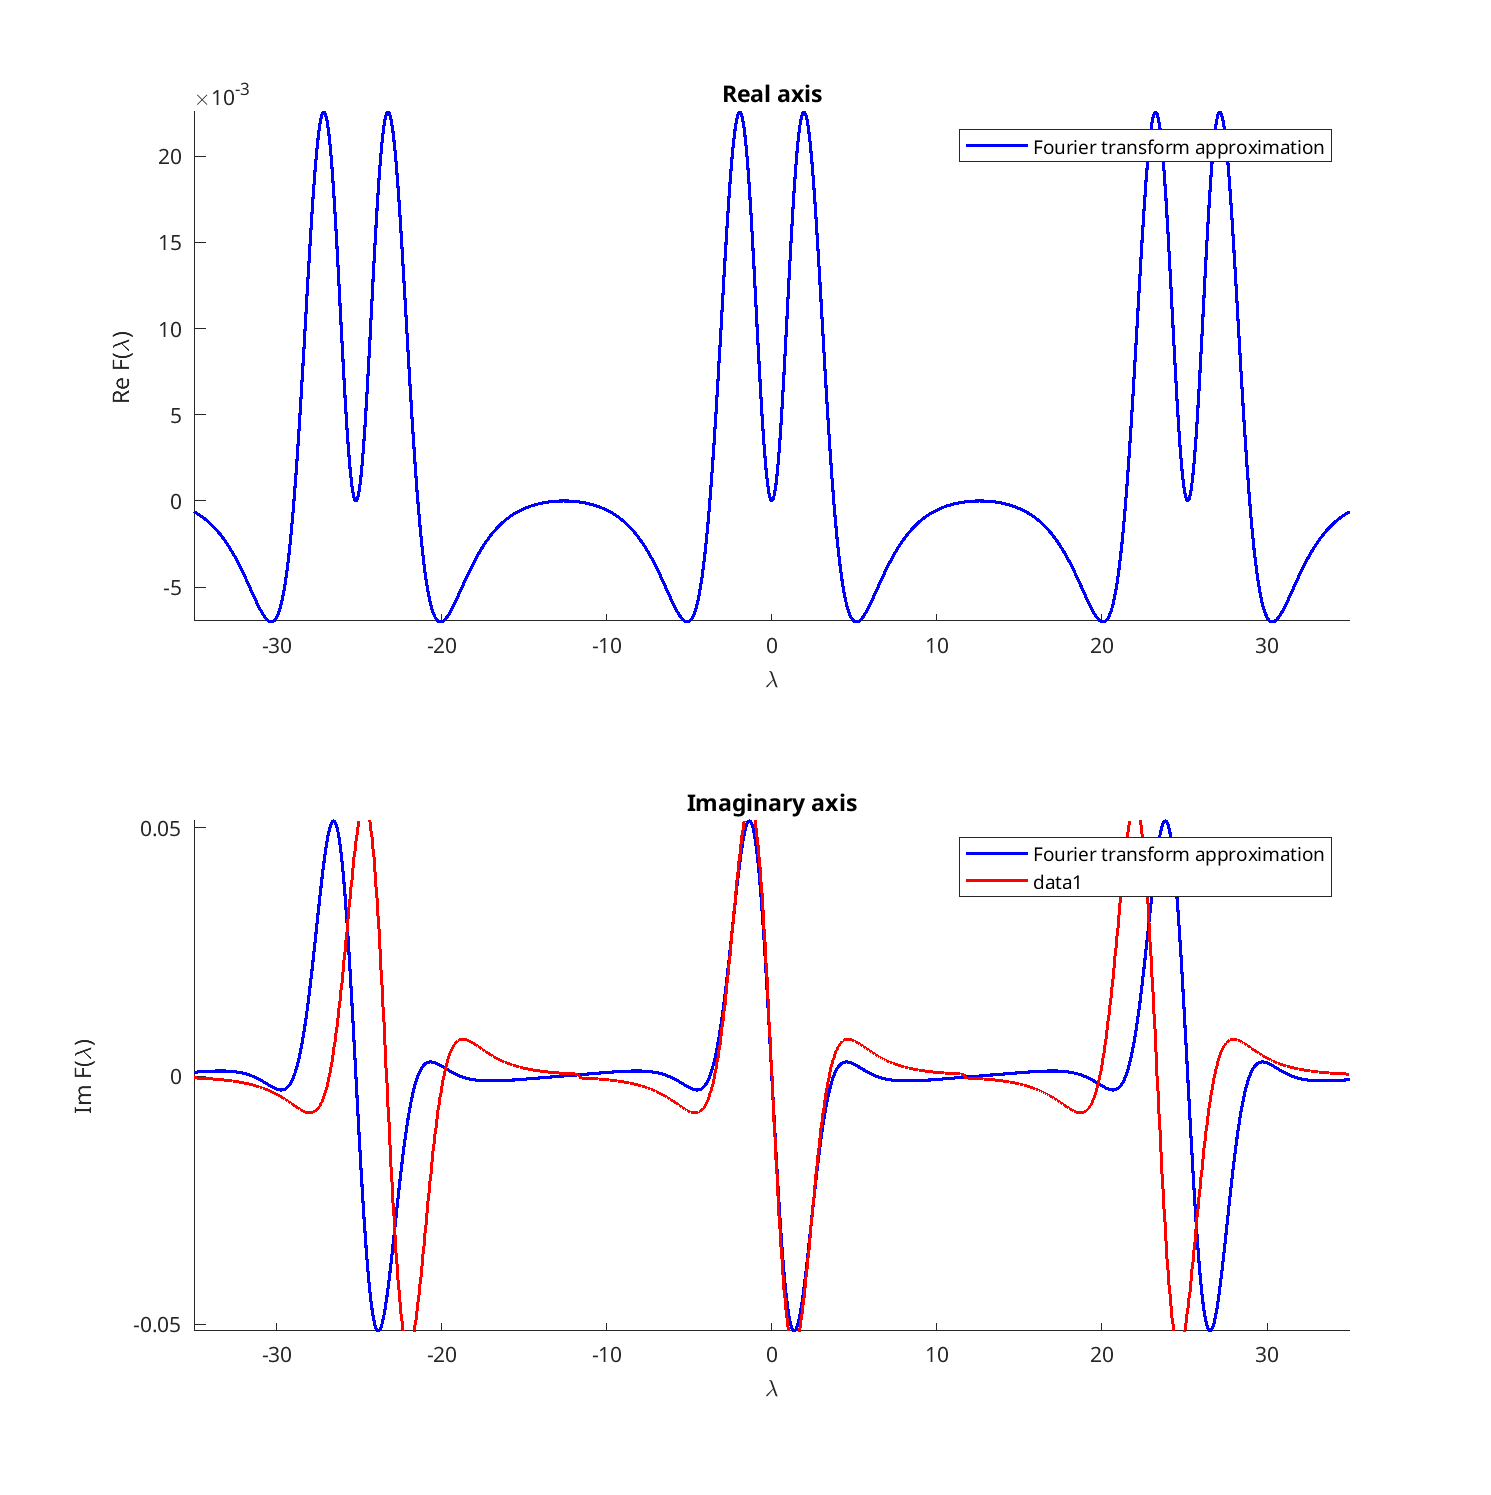
\includegraphics[width=\textwidth, height=0.5\textheight]{Aliasing-3}
\caption{$ T = 100, \Delta t = 0.25 $}
\end{figure}

\newpage

\begin{figure}[h]
\centering
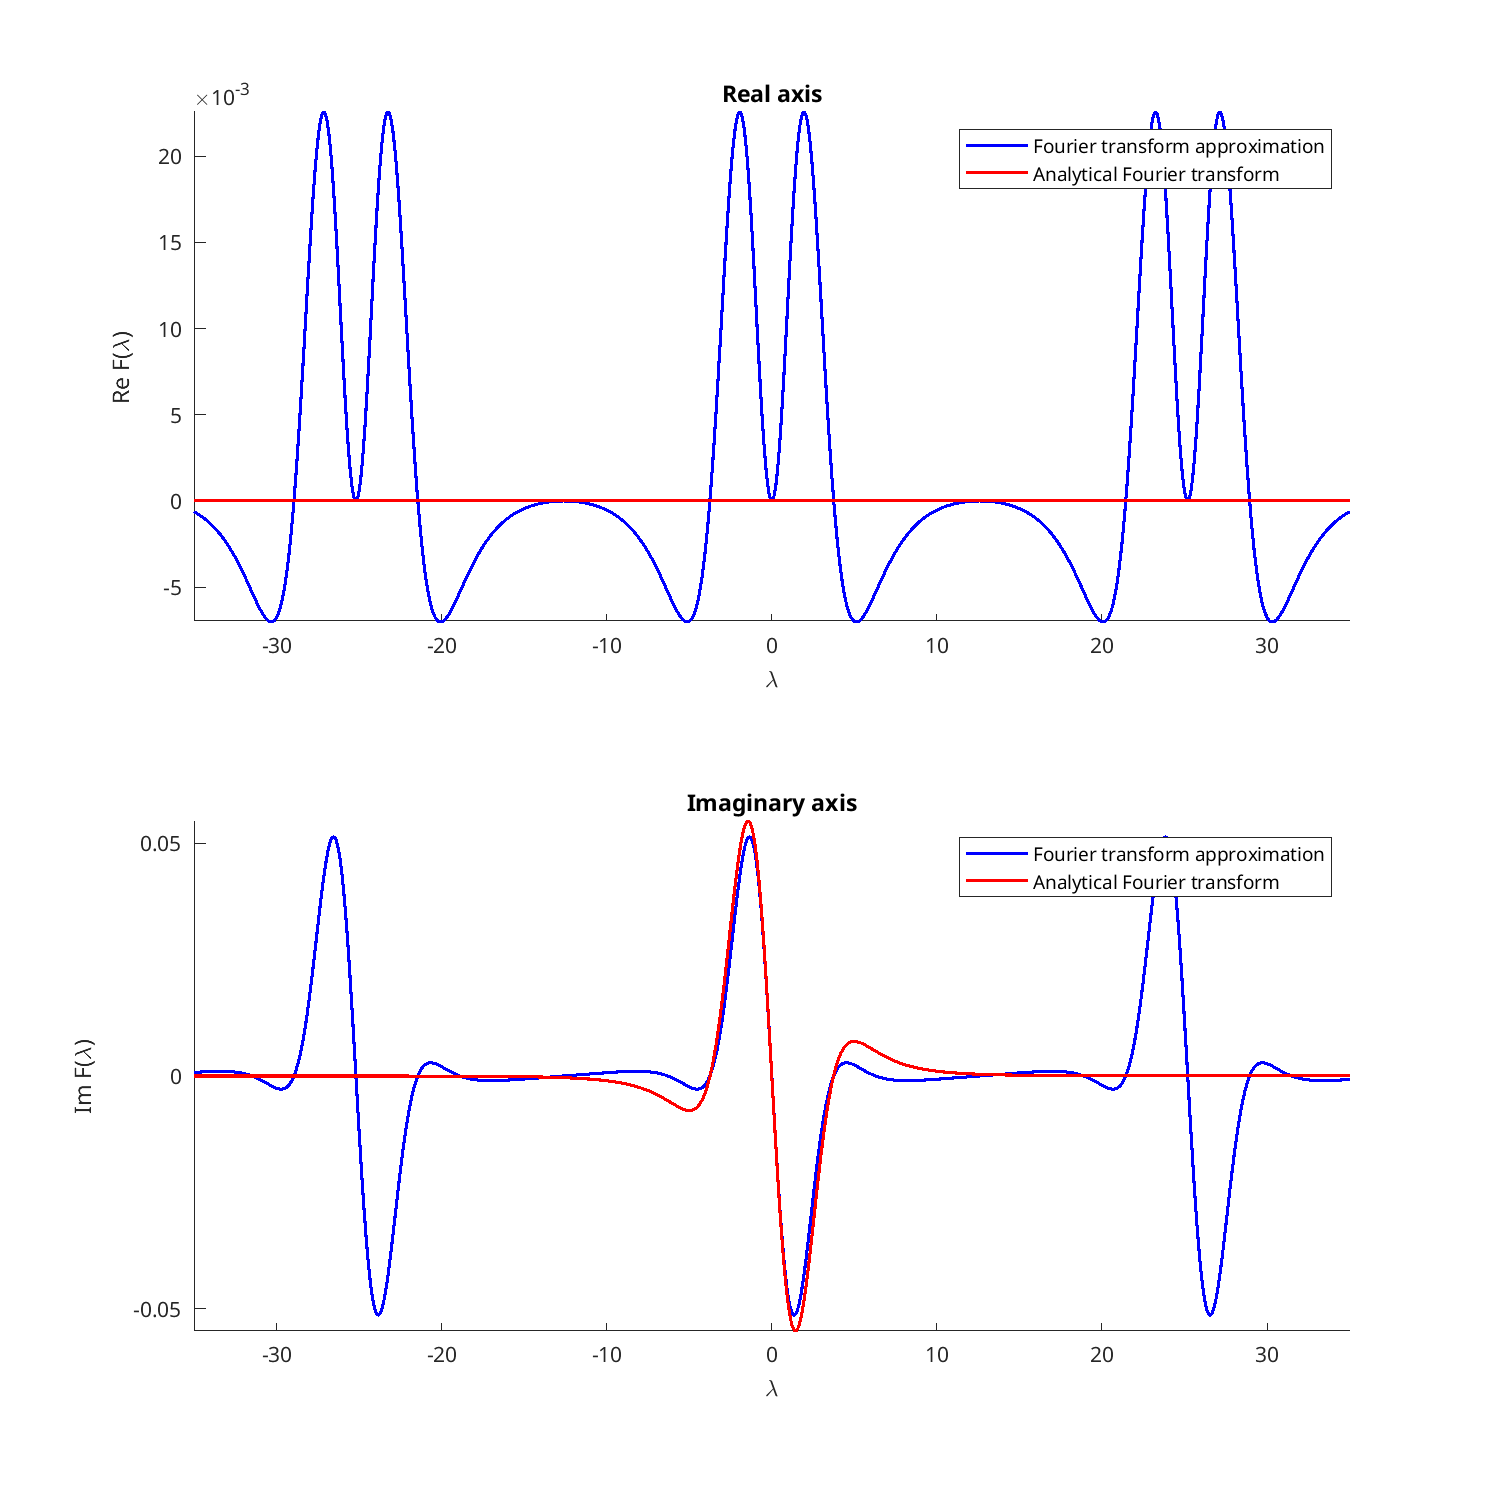
\includegraphics[width=\textwidth, height=0.35\textheight]{Aliasing}
\caption{$ T = 100, \Delta t = 0.25 $}
\end{figure}

\begin{figure}[h]
\centering
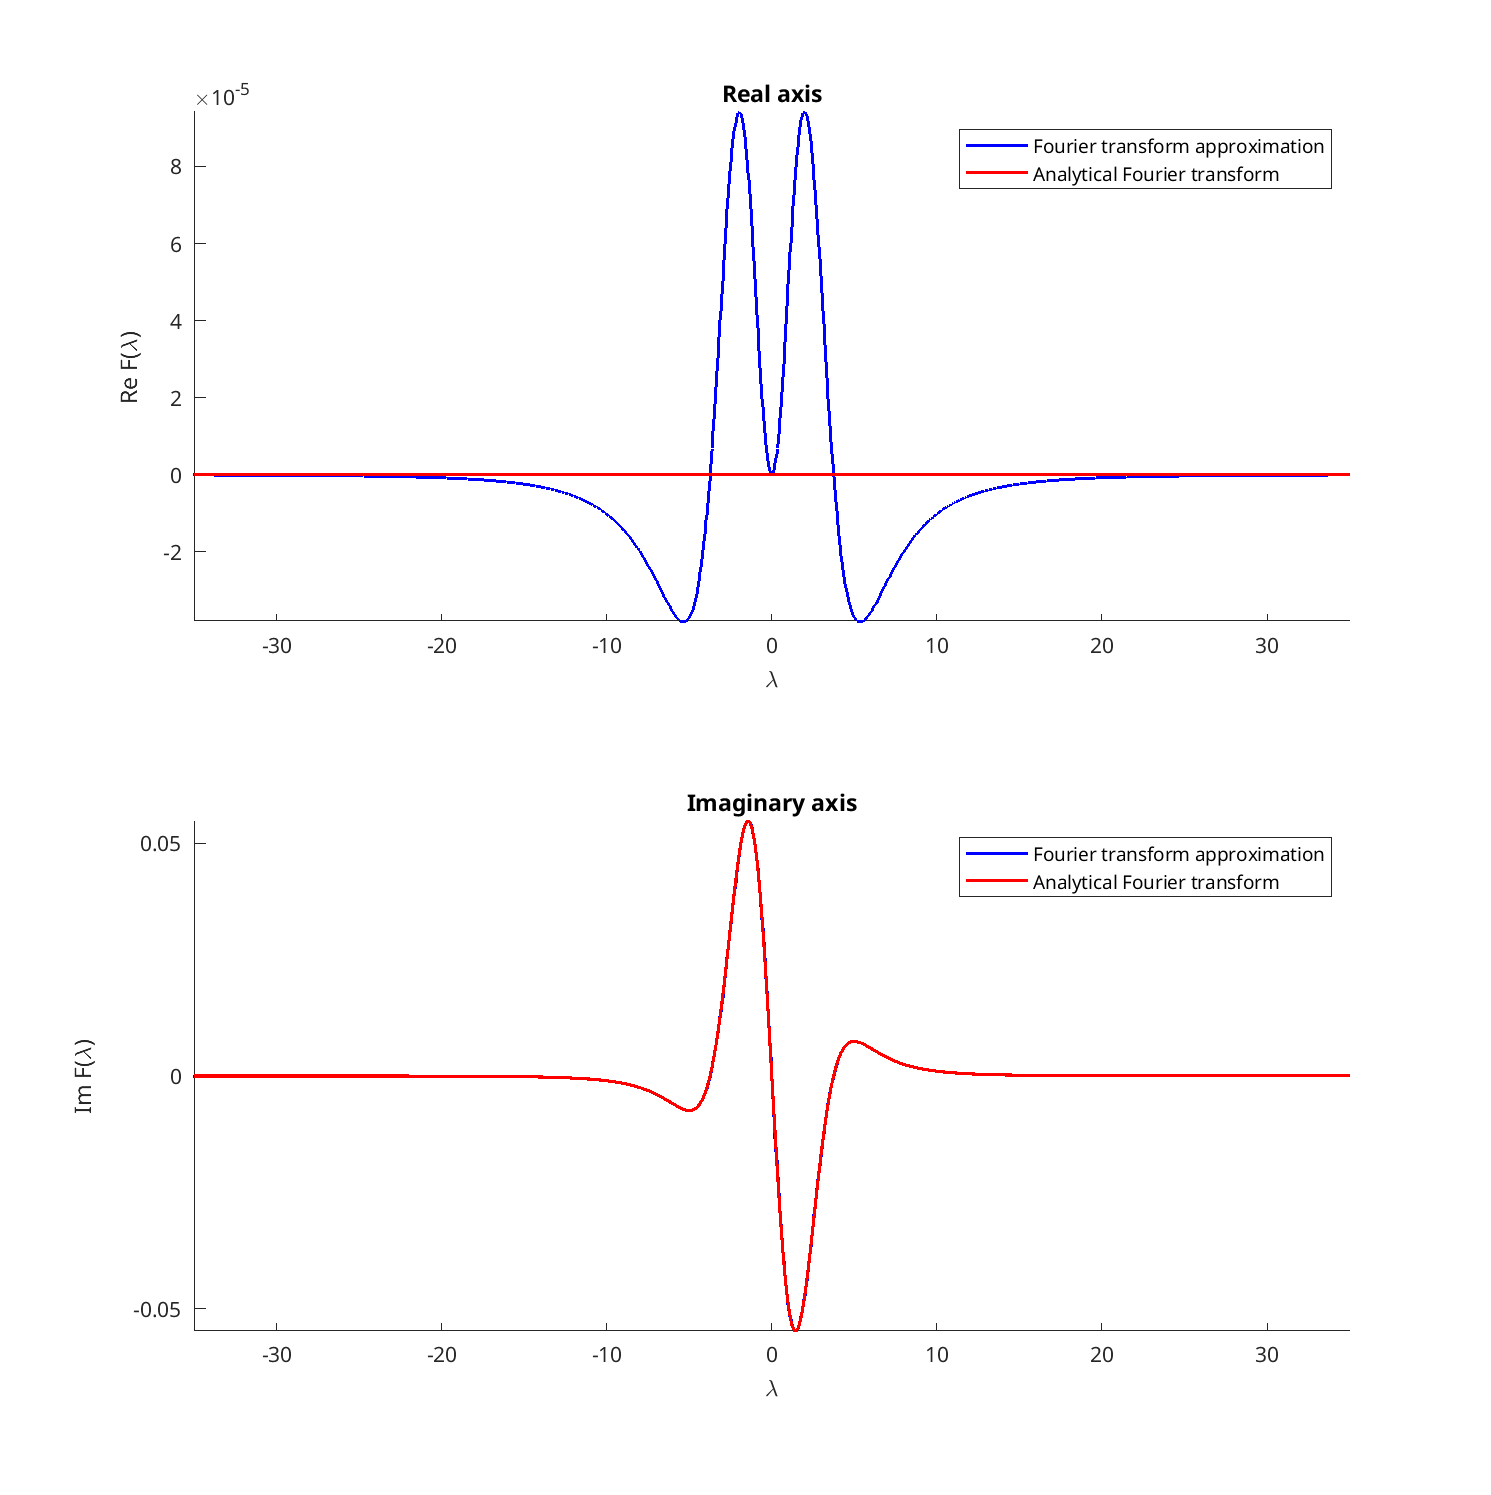
\includegraphics[width=\textwidth, height=0.35\textheight]{Aliasing-2}
\caption{$ T = 500, \Delta t = 10^{-3} $}
\end{figure}